%%%%%%%%%%%%%%%%%%%%%%%%%%%%%%%%
\subsection{Objetivos}
% ----------------------------------------------------------------------------
\begin{frame}{Reconhecimento de Voz}

\begin{figure}
	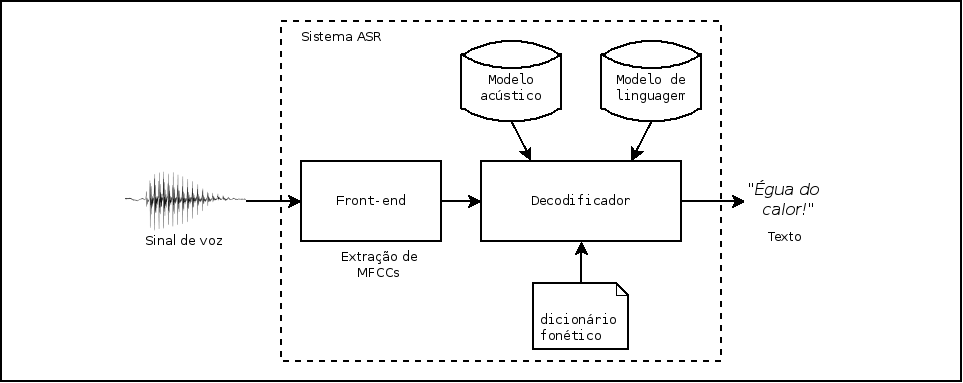
\includegraphics[width=0.5\textwidth]{Figures/asr}
    \caption{Esquema tradicional de um sistema autom\'atico de reconhecimento de voz}
\end{figure}

\begin{itemize}
    \item Aplica\c c\~oes:
    \begin{itemize}
        \smallskip
		\item Tecnologias assistivas, \textit{eye-trackers}, lingu\'istica (\textbf{alinhamento fon\'etico}), s\'intese de voz
    \end{itemize}
\end{itemize}
\end{frame}

\begin{frame}{Ferramentas Utilizados}
    \begin{itemize}
        \item Kaldi: um pacote \textit{open-source} de reconhecimento de voz
			\begin{itemize}
				\item Possui suporte para ambas HMM-GMMs (mistura de gaussianas) e HMM-DNNS (redes neurais profundas)
				\item Suporte para PT-BR
			\end{itemize}
		\begin{figure}
		\begin{center}
			
\includegraphics[width=0.4\textwidth]{Figures/kaldi}
		\end{center}
		\end{figure}

        \item Praat: \textit{software} utilizado por linguistas na  an\'alise da fala

    \end{itemize}
\end{frame}


\begin{frame}{Objetivos}
\begin{itemize}
    \item Desenvolver um sistema de reconhecimento de voz para PT\_BR utilizando o pacote Kaldi para treinamento dos AMs e LMs
\end{itemize}

\begin{itemize}
    \item Disponibilizar recursos \`a comunidade cient\'ifica
\end{itemize}
\begin{figure}
\begin{center}
	
\includegraphics[width=0.3\textwidth]{Figures/falabrasil}
\end{center}
\end{figure}

\end{frame}
